\documentclass[12pt]{article}
\usepackage[utf8]{inputenc}
\usepackage[T2A]{fontenc}
\usepackage[russian]{babel}
\usepackage{amsmath}
\usepackage{amssymb}
\usepackage{dsfont}
\usepackage[dvipsnames]{xcolor}
\usepackage{setspace}
\usepackage{multirow}
\usepackage[a4paper, outer=1.5cm, inner=1.5cm, top=1cm, bottom=1cm]{geometry}
\usepackage{graphicx}
\usepackage{skull}
\usepackage{wasysym}
\usepackage{float}
\graphicspath{{.images/}}
\usepackage{hyperref}
\hypersetup{colorlinks=true, linkcolor=blue, filecolor=magenta, urlcolor=cyan}
\usepackage[firstpage]{draftwatermark}
\SetWatermarkText{
    $\qquad\qquad\qquad\qquad\qquad$\parbox{7cm}{\begin{center}
    
\includegraphics[width = 0.08\textwidth]{lion-logo.png}\bigskip\\~\bigskip\\~\vspace{-24mm}\\~\end{center}}
}
\SetWatermarkAngle{0}
\SetWatermarkScale{1.5}
\usepackage{etoolbox}

\newtoggle{ifsolved}
\newtoggle{needhelp}
\newcounter{num}
\setcounter{num}{1}

\newcommand{\newnum}{\par\textbf{\textnumero\arabic{num}}\stepcounter{num}}
\newcommand{\sol}{\vspace{3mm}\par\textbf{Решение: }}
\newcommand{\ans}{\vspace{3mm}\par\textbf{Ответ: }}
\newcommand{\hint}{\vspace{3mm}\par\textbf{Подсказка: }}
\newcommand{\mode}[1]{
\ifstrequal{#1}{0}{\togglefalse{ifsolved}\togglefalse{needhelp}}{\ifstrequal{#1}{1}{\togglefalse{ifsolved}\toggletrue{needhelp}}{\ifstrequal{#1}{2}{\toggletrue{ifsolved}\togglefalse{needhelp}}{\toggletrue{ifsolved}\toggletrue{needhelp}}}}} %if 0 - if 1 - if 2 - else
%\newenvironment{problem}[8]{%#1, #2, #3
%\parbox{\linewidth}{\vspace{4mm}\ifstrequal{#4}{(лёгкая)}{\newnum\textbf{.}}{\newnum\textbf{*.} } \\ #5}
%\iftoggle{ifsolved}{\sol #6}{}
%\iftoggle{ifsolved}{\ans #7}{}
%\iftoggle{needhelp}{\hint #8}{}}

\newenvironment{problem}[8]{%#1, #2, #3
\parbox{\linewidth}{\vspace{5mm}\ifstrequal{#4}{(лёгкая)}{\newnum\textbf{.}}{\newnum\textbf{*.} } \\ #5}
\iftoggle{ifsolved}{\sol #6}{}

\iftoggle{ifsolved}{\parbox{\linewidth}{\ans #7}}{}
\iftoggle{needhelp}{\parbox{\linewidth}{\hint #8}}{}}

\newenvironment{mylist} %custom list
{ \begin{itemize}
    \setlength{\itemsep}{0pt}
    \setlength{\parskip}{0pt}
    \setlength{\parsep}{0pt}     }
{ \end{itemize}                  }

\newenvironment{homeass}[1]{\vspace*{-1.5cm}
\iftoggle{ifsolved}{
    \section*{\center{Решение домашнего задания к #1.}}
}{
    \section*{\center{\textcolor{Sepia}{Домашнее задание к #1}}}
} \vspace{7mm}\large}

\parindent=0pt
\pagestyle{empty}
%$\!$[\arabic{class}.\arabic{num}]
%\ifnumcomp{\value{counter}}{>}{1}{true}{false}
%\definecolor{Gray}{gray}{0.9}
%\definecolor{mypink}{RGB}{219, 48, 122}
%\newcolumntype{g}{>{\columncolor{Gray}}p{2.8cm}}

\begin{document}
\large
\mode{7}
%0 for problems without hints
%1 for problems + hints
%2 for problems + solutions + answers
%else: show all

{\centering\section*{СПИСОК ЗАДАЧ}}

{\centering\subsection*{\smallskip\\\textcolor{green}{\textbf{Полезные вещи, которые можно и нужно копипастить:}}}}

\subsection*{\textcolor{Emerald}{\textbf{Полезные шпаргалки по LaTeXу:}}}

\textbf{Пример вставки рисунка:}

\begin{minipage}{\linewidth}
    \begin{minipage}{0.54\linewidth}
    см. рисунок справа\\
    Текст к собственно пикче, примерно всегда это либо развёрнутое описание, либо большая часть решения задачи --- стремимся экономить пространство, если это можно сделать.
    \end{minipage}
    \hspace{0.05\linewidth}
    \begin{minipage}{0.4\linewidth}
    \begin{figure}[H] 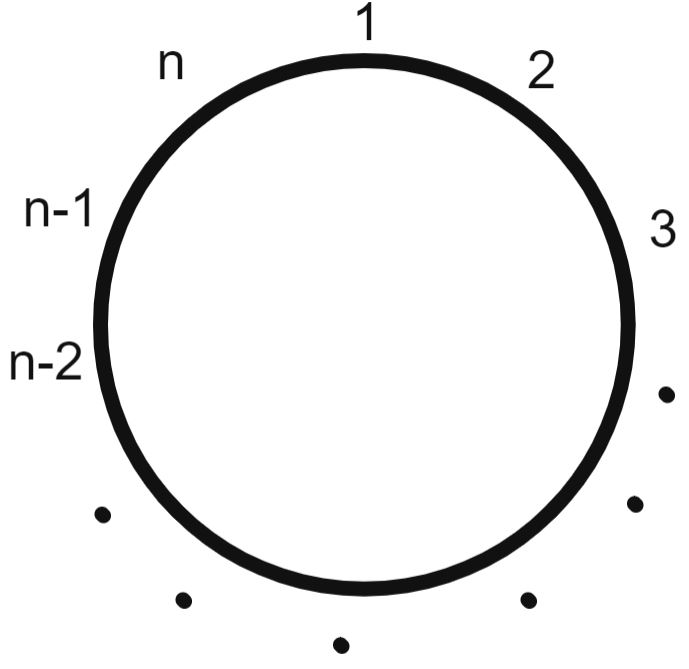
\includegraphics[width=\linewidth]{sol3} %тут поменять имя пикчи
    \end{figure}
    \end{minipage}
\end{minipage}

\textbf{Дефолтные математические знаки и символы:}\\
$\geqslant$,
$\leqslant$,
$a^{b}$,
$x_{i}$,
$\sqrt{a}$,
$\frac{a}{b}$,
$\displaystyle \frac{a}{b}$,
$\cdot$
$\;\Rightarrow\;$,
$\;\Leftrightarrow\;$,
$1{,}2$.
О промежутках:
$a\!b$,
$a\,b$,
$a\:b$,
$a\;b$,
$a\quad b$.

\textbf{Стандартные система и совокупность уравнений / неравенств:}\\
$\left\{
\begin{aligned}
f(x) &= 0 \\
g(x) &= 1
\end{aligned}\right.$

$\left[\begin{aligned}
&\left\{\begin{aligned}
f(x) &\geqslant a \\
g(x) &= b
\end{aligned}\right.\\
&\left\{\begin{aligned}
f(x) &< a \\
g(x) &= -b
\end{aligned}\right.
\end{aligned}\right.$

\subsection*{\textcolor{Emerald}{\textbf{Не математическое, но полезное:}}}
% комментарий в любом месте документа, который нигде не будет видно. Можно использовать для написания заметок-вопросов по задачам
\textbf{Пример таблицы:}

\begin{tabular}{|c|c|c|}
\hline
    $a$ & $b$ & текст
\\\hline
    $c$ & $d$ & мораль
\\\hline
\end{tabular}\\

\textbf{Отступы:} между\smallskip\\ строками\medskip\\ \textbf{Тире} --- это три дефиса.\\
\textbf{Списки:}
\begin{mylist}
\item [$\bullet$] это был пункт а
\item [2)] а это уже пункт номер 2 с изменённым заголовком
\end{mylist}

\subsection*{\textcolor{Emerald}{\textbf{Всё, неупомянутое выше (или если просто что-то не так):}}}
\begin{mylist}
\item [$\bullet$] Решение отдельных вопросов касательно ТеХа нужно искать в \href{https://www.mccme.ru/free-books/llang/newllang.pdf}{Львовском}.

\item [$\bullet$] Найти произвольный символ, который нужен, можно в \href{http://detexify.kirelabs.org/classify.html}{Detexify}.

\item [$\bullet$] Если возникли сомнения при решении, ответ практически ко всем задачам можно проверить с помощью \href{https://www.wolframalpha.com/}{WolframAlpha}.

\item [$\bullet$] Если в задаче нужно создать картинку, то лучше пока отложить эту задачу. Все графики планируется централизованно нарисовать (или перерисовать) в геогебре.

\item [\textcolor{brown}{\textbf{!!}}] Важно ставить \textcolor{red}{\textbf{$\spadesuit$}}
(или просто red) в тело задачи в случае серьёзных вопросов к решению и какой-то вопиющей лажи.

\item [\textcolor{brown}{\textbf{!!}}] Важно ставить \textcolor{olive}{\textbf{$\spadesuit$}}
(или просто olive) в тело задачи в случае не самого удачного текста и кривых отступов.
\end{mylist}

\subsection*{\textcolor{Violet}{\textbf{Комментарии:}}}% а также невидимые комментарии - так можно оставлять заметки-вопросы прямо в задаче, чтобы потом было понятно, в чём вопрос.
\begin{mylist}
\item [$\skull$] Переставлять задачи местами --- очень плохая идея.

\item [$\smiley$] При двойном клике по тексту pdf справа происходит автоматический переход к этому месту в латех-коде, а для обратного перехода можно нажать стрелку вправо (висит сверху между pdf и латех-кодом).

\item [$\smiley$] Если есть размышления, дописывать red/olive к задаче или не дописывать, то лучше всё-таки дописать.

\item [$\skull$] Самое плохое, что можно сделать --- написать в любое поле из трёх (НаписанноеРешение/ВерныйОтвет/Подсказка) только половину того, что надо, никак это не отметить, и потом пойти дальше.\\ Нужно в этот момент писать red/olive в случайном месте задачи, чтобы потом вычислить это с помощью Ctrl+F по всему документу (и это то, что потом будет делаться долго и тщательно)
\end{mylist}

\newpage
\setcounter{num}{1072}

\hypertarget{9.1}{{\centering\section*{\bigskip\\\textcolor{Blue}{\hyperlink{start2}{\textcolor{Blue}{9.1}} Неравенства.}\vspace{-5mm}}}}

\begin{problem}{Линейные неравенства.}{9.1.1}{X}{(лёгкая)}
{Найти наибольшее целое решение неравенства $\,\displaystyle x - \frac{x - 1}{2} - \frac{x + 3}{4} < 2$.}
{НаписанноеРешение}
{ВерныйОтвет}{Подсказка}
\end{problem}

\begin{problem}{Линейные неравенства.}{9.1.1}{9I}{(лёгкая)}
{Найти наименьшее целое решение неравенства $\,-(4x - 5)^{2} \geqslant (2x + 3)(5 - 8x)$.}
{НаписанноеРешение}
{ВерныйОтвет}{Подсказка}
\end{problem}

\begin{problem}{Линейные неравенства.}{9.1.1}{X}{(лёгкая)}
{Пусть $\alpha$ и $\beta$ --- углы треугольника. Известно, что $58^{\circ}\leqslant \alpha \leqslant59^{\circ}$, $102^{\circ}\leqslant \beta \leqslant103^{\circ}$.\\
Оценить с помощью неравенств величину третьего угла.}
{Если бы мы точно знали два угла треугольника, третий угол мог бы быть найден как $\gamma = 180^{\circ} - (\alpha + \beta)$ по формуле для суммы углов треугольника. Понятно, что $\alpha + \beta \geqslant 160^{\circ}$ и $\alpha + \beta \leqslant 162^{\circ}$. Тогда имеем двойное неравенство $-162^{\circ} \leqslant -(\alpha + \beta) \leqslant -160^{\circ}$, а значит, $180^{\circ} - 162^{\circ} \leqslant 180^{\circ} - (\alpha + \beta) \leqslant 180^{\circ} - 160^{\circ}$.
Таким образом, $18^{\circ} \leqslant \gamma \leqslant 20^{\circ}$.}
{Третий угол треугольника может принимать значения от $18^{\circ}$ до $20^{\circ}$.}{Какой может быть сумма этих двух углов?}
\end{problem}

\begin{problem}{Линейные неравенства.}{9.1.1}{X}{(лёгкая)}
{Оценить сумму, разность, произведение, и частное чисел $a$ и $b$, если известно, что $3 < a < 4\:$ и $\:6 < b < 9$.}
{Понятно, что сумма чисел будет наибольшей, если числа больше, и наименьшей, если числа меньше. Поэтому $9 < a + b < 13$.

Разность чисел $a$ и $b$ будет больше, если $a$ побольше, а $b$ поменьше, и будет меньше, если наоборот. То есть $-6 < a - b < -2$.

Поскольку все числа положительны, произведение будет больше при больших числах $a$ и $b$ и меньше --- при меньших. Поэтому $18 < ab < 36$.

Опять же, так как все числа положительны, частное будет наибольшим, если $a$ большое, а $b$ маленькое, и наименьшим, если наоборот, $a$ маленькое, а $b$ большое. Следовательно, $\frac{1}{3} < \frac{a}{b} < \frac{2}{3}$.}
{$\,9 < a + b < 13$; $\quad-6 < a - b < -2$; $\quad18 < ab < 36$; $\quad\frac{1}{3} < \frac{a}{b} < \frac{2}{3}$.}{Аккуратно рассмотреть все основные случаи и убедиться, что ничего не упущено. Наибольшие и наименьшие варианты для каждой арифметической операции разные.}
\end{problem}

\begin{problem}{Линейные неравенства.}{9.1.1}{X}{*}
{Оценить сумму, разность, произведение, и частное чисел $n$ и $p$, если известно, что $-5 < n < -2\:$ и $\:1 < p < 4$.}
{Понятно, что сумма чисел будет наибольшей, если числа побольше, и наименьшей, если числа поменьше. Поэтому $-4 < n + p < 2$.

Разность чисел $n$ и $p$ будет наибольшей, если $n$ побольше, а $p$ поменьше, и будет меньше, если наоборот. То есть $-9 < n - p < -3$.

Поскольку первое число гарантированно отрицательно, а второе гарантированно положительно, произведение будет меньше при числах, больших по модулю, и меньше --- при числах, меньших по модулю. Поэтому $-20 < np < -2$.

Опять же, так как дробь будет отрицательна, частное будет наибольшим, если $n$ велико по модулю, а $p$ мало, и наименьшим, если наоборот, $p$ мало по модулю, а $p$ велико. Следовательно, $-5 < \frac{n}{p} < -\frac{1}{2}$.}
{$\,-4 < n + p < 2$; $\quad-9 < n - p < -3$; $\quad-20 < np < -2$; $\quad-5 < \frac{n}{p} < -\frac{1}{2}$.}{Аккуратно рассмотреть все основные случаи и убедиться, что ничего не упущено. Следует учесть, что наибольшие и наименьшие варианты для каждой арифметической операции разные, а также что при умножении и при делении в итоге получится отрицательное число.}
\end{problem}

\begin{problem}{Линейные неравенства.}{9.1.1}{X}{(лёгкая)}
{Нарисовать на координатной прямой решения двойного неравенства $$6 - 3 < x < 6 + 3.$$ Почему логично называть данное множество окрестностью точки $O$ с радиусом $r$? Как ты думаешь, где находится на полученном рисунке точка $O$, и каков радиус у этой окрестности?}
{На координатной прямой ниже можно увидеть решение.
\vspace{-4mm}\\\begin{minipage}{\linewidth}
\begin{figure}[H] 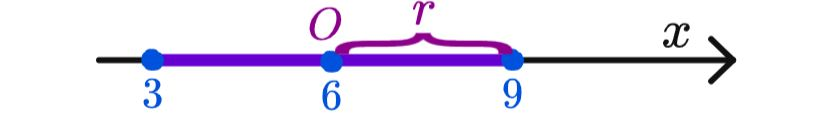
\includegraphics[width=\linewidth]{sol82}\end{figure}
\end{minipage}
Понятно, что все точки на рисунке, являющиеся решениями, представляют собой множество точек, который отличаются от 6 не более чем на 3. То есть, интуитивно ясно, что можно называть данное множество <<точками возле $x_0 = 6$>>.\\
Точка $O$ здесь имеет координату 6, а радиус этой <<окрестности>> --- 3.}
{Смотри рисунок выше. Также это можно записать короче как $|x - x_0| < r$.}{Отметь на координатной прямой $x = 3$ и $x = 9$.}
\end{problem}

\begin{problem}{Линейные неравенства.}{9.1.1}{9I}{*}
{Найти наименьшее целое решение неравенства $\,(2 - \sqrt{5})x < 2 + \sqrt{5}$.}
{НаписанноеРешение}
{ВерныйОтвет}{Подсказка}
\end{problem}

\begin{problem}{Линейные неравенства.}{9.1.1}{9I}{*}
{Найти наибольшее целое решение неравенства $\,(3 - \sqrt{10}) \cdot x \geqslant 3 + \sqrt{10}$.}
{НаписанноеРешение}
{ВерныйОтвет}{Подсказка}
\end{problem}

\begin{problem}{Линейные неравенства.}{9.1.1}{9I}{*}
{Найти наименьшее целое решение неравенства $\,(17 - \sqrt{1003}) \cdot x < 5 + \sqrt{73}$.}
{НаписанноеРешение}
{ВерныйОтвет}{Подсказка}
\end{problem}

\begin{problem}{Линейные неравенства.}{9.1.1}{9I}{*}
{Найти наибольшее целое решение неравенства $\,(12 + \sqrt{227}) \cdot x < 17 + \sqrt{666}$.}
{НаписанноеРешение}
{ВерныйОтвет}{Подсказка}
\end{problem}

\begin{problem}{Линейные неравенства.}{9.1.1}{9I}{*}
{Найти наибольшее целое решение неравенства $\,(6 - \sqrt{20}) \cdot x \leqslant (6 + \sqrt{20})$.}
{НаписанноеРешение}
{ВерныйОтвет}{Подсказка}
\end{problem}

\begin{problem}{Квадратные неравенства.}{9.1.2}{79I}{(лёгкая)}
{Нарисовать график параболы $y = x^{2} - 6x - 7$ и решить квадратное неравенство $\displaystyle x^{2} - 6x - 7 < 0$.}
{НаписанноеРешение}
{ВерныйОтвет}{Подсказка}
\end{problem}

\begin{problem}{Квадратные неравенства.}{9.1.2}{79I}{(лёгкая)}
{Нарисовать нужные графики и решить квадратное неравенство $\displaystyle x^{2} \leqslant -20 + 9x$.}
{НаписанноеРешение}
{ВерныйОтвет}{Подсказка}
\end{problem}

\begin{problem}{Квадратные неравенства.}{9.1.2}{79I}{(лёгкая)}
{Камнеметательная машина стреляет камнями под некоторым углом к горизонту.\\ Траектория полёта камня описывает формулой $\displaystyle y = ax^{2} + bx$, где $a = -\frac{1}{600}$, $\,b = \frac{4}{15}$,\\ $x$~--- смещение камня по горизонтали~(м), $y$~--- высота камня над землёй (м).\\ На каком наибольшем расстоянии от крепостной стены высотой 9 метров можно расположить машину, если необходимо, чтобы камни пролетали над стеной на высоте как минимум 1 метр?}
{НаписанноеРешение}
{ВерныйОтвет}{Подсказка}
\end{problem}

\begin{problem}{Квадратные неравенства.}{9.1.2}{79I}{(лёгкая)}
{a) Определить, существуют ли такие $x$, что $\displaystyle x^{2} + 10 < 6x$.
\\b) Определить, существуют ли такие $x$, что $\displaystyle x^{2} + 10 < 7x$.}
{НаписанноеРешение}
{ВерныйОтвет}{Подсказка}
\end{problem}

\begin{problem}{Квадратные неравенства.}{9.1.2}{79I}{(лёгкая)}
{Решить квадратное неравенство $\displaystyle (2x + 1)(x - 3) < x^{2} + 21$.}
{НаписанноеРешение}
{ВерныйОтвет}{Подсказка}
\end{problem}

\begin{problem}{Квадратные неравенства.}{9.1.2}{79I}{(лёгкая)}
{Какое из квадратных неравенств не имеет решений?
\\1) $\displaystyle x^{2} - 4x - 11 < 0$
\hspace*{4cm} 2) $\displaystyle x^{2} - 4x - 11 > 0$
\\3) $\displaystyle x^{2} - 4x + 11 < 0$
\hspace*{4cm} 4) $\displaystyle x^{2} - 4x + 11 > 0$}
{В каждом из этих четырёх неравенств выражение слева --- квадратный трёхчлен, для которого соответствующая парабола имеет ветви, направленные вверх (так как старший коэффициент $a$ равен 1). Поэтому неравенства 2) и 4) решения, очевидно, имеют --- рано или поздно получится найти какие-то положительные значения. Решений у неравенств 1) и 3) может не быть, если график соответствующей параболы находится выше оси абсцисс, то есть имеет менее 2 корней (если два корня есть, то парабола между ними принимает отрицательные значения). Квадратное уравнение не имеет двух корней, если $D \leqslant 0$. В первом случае $D = (-4)^2 - 4\cdot(-11) = 16 + 44 = 60 > 0$, корни у уравнения есть, и решения у неравенства найдутся. В третьем же случае $D = (-4)^2 - 4\cdot(11) = 16 - 44 = -26 < 0$. Тогда решений у уравнения и у неравенства нет, что и требовалось.}
{Решений не имеет неравенство \textnumero3, $\,x^{2} - 4x + 11 < 0$.}{Направление ветвей параболы $+$ знак дискриминанта.}
\end{problem}

\begin{problem}{Квадратные неравенства.}{9.1.2}{79I}{(лёгкая)}
{Решить квадратное неравенство $\displaystyle x^{2} - 4x - 21 > 0$.}
{НаписанноеРешение}
{ВерныйОтвет}{Подсказка}
\end{problem}

\begin{problem}{Квадратные неравенства.}{9.1.2}{79I}{(лёгкая)}
{Решить квадратное неравенство $\displaystyle 12x + 32 \leqslant -x^{2}$.}
{НаписанноеРешение}
{ВерныйОтвет}{Подсказка}
\end{problem}

\begin{problem}{Квадратные неравенства.}{9.1.2}{79I}{(лёгкая)}
{Решить квадратное неравенство $\displaystyle 2(x^{2} + 44) < 27x$.}
{НаписанноеРешение}
{ВерныйОтвет}{Подсказка}
\end{problem}

\begin{problem}{Квадратные неравенства.}{9.1.2}{79I}{(лёгкая)}
{Решить квадратное неравенство $\displaystyle (2s + 3)(s - 1) \leqslant 0$.}
{НаписанноеРешение}
{ВерныйОтвет}{Подсказка}
\end{problem}

\begin{problem}{Квадратные неравенства.}{9.1.2}{79I}{(лёгкая)}
{Решить квадратное неравенство $\displaystyle x^{2} - x - 30 < 0$.}
{НаписанноеРешение}
{ВерныйОтвет}{Подсказка}
\end{problem}

\begin{problem}{Квадратные неравенства.}{9.1.2}{79I}{(лёгкая)}
{Решить квадратное неравенство $\displaystyle 2x^{2} + 65 \geqslant 23x$.}
{НаписанноеРешение}
{ВерныйОтвет}{Подсказка}
\end{problem}

\begin{problem}{Квадратные неравенства.}{9.1.2}{79I}{(лёгкая)}
{Решить квадратное неравенство $\displaystyle 2x^{2} + x < 55$.}
{НаписанноеРешение}
{ВерныйОтвет}{Подсказка}
\end{problem}

\begin{problem}{Квадратные неравенства.}{9.1.2}{79I}{(лёгкая)}
{Решить квадратное неравенство $\displaystyle x^{2} - 2x - 63 \leqslant 0$.}
{НаписанноеРешение}
{ВерныйОтвет}{Подсказка}
\end{problem}

\begin{problem}{Квадратные неравенства.}{9.1.2}{79I \textcolor{olive}{\textbf{$\spadesuit$}}}{(лёгкая)}
{\vspace{-12mm}\\\begin{minipage}{\linewidth}
    \begin{minipage}{0.5\linewidth}

    На рисунке справа изображены графики параболы и прямой.\\
    1) Найти точки их пересечения с помощью алгебраических методов.\\
    2) Сколько натуральных чисел являются решениями неравенства $x^{2} - 13x + 42 < 35 - 5x$?

    \end{minipage}
    \hspace{0.05\linewidth}
    \begin{minipage}{0.44\linewidth}
        \begin{figure}[H]
        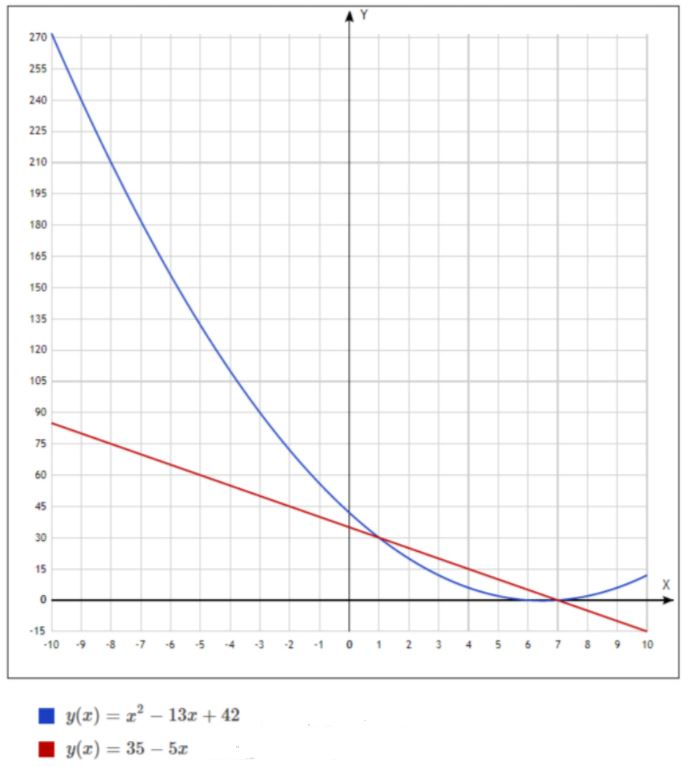
\includegraphics[width=\linewidth]{79I-1}
        \end{figure}
    \end{minipage}
\end{minipage}}
{Там, где прямая пересекается с параболой, $x^2 - 13x + 42 = y = 35 - 5x$.
Поэтому $x^2 - 13x + 42 = 35 - 5x \;\Rightarrow\; x^2 - 8x + 7 = 0 \;\Rightarrow\; (x - 1)(x - 7) = 0$. Следовательно, $x = 1$ или $x = 7$.

Находим ординаты обеих точек пересечения: $y_1 = 35 - 5\cdot1 = 30 \;\Rightarrow\; (1; 30)$ и $y_2 = 35 - 5\cdot7 = 0 \;\Rightarrow\; (7; 0)$. Итого, точки пересечения --- точки $(1; 30)$ и $(7; 0)$.\smallskip\\
Решаем неравенство: $$x^{2} - 13x + 42 < 35 - 5x \;\Rightarrow\; x^2 - 8x + 7 < 0 \;\Rightarrow\; (x - 1)(x - 7) < 0.$$ Произведение двух чисел может быть меньше 0 в том и только том случае, если одно из них положительно, а другое отрицательно. Поэтому $1 < x < 7$.

То есть между найденными нами ранее точками пересечения прямой и параболы. Действительно, неравенство требует условие <<значение параболы меньше значения прямой>>, то есть <<на графике прямая находится выше параболы>>. Натуральные числа на этом промежутке --- 2, 3, 4, 5, 6 (сами 1 и 7 решениями неравенства уже не являются).}
{Парабола и прямая пересекаются в точках $(1; 30)$ и $(7; 0)$.\\ Натуральные числа, являющиеся решениями неравенства --- числа 2, 3, 4, 5, 6.}{Уравнение решается как обычно, а для решения неравенства достаточно только решить уравнение (и понять, почему этого достаточно).}
\end{problem}

\begin{problem}{Квадратные неравенства.}{9.1.2}{79I red четвертая степень + корни не +-1 в метод интервалов \textcolor{olive}{\textbf{$\spadesuit$}}}{*}
{\vspace{-6mm}\\\begin{minipage}{\linewidth}
    \begin{minipage}{0.5\linewidth}

    На рисунке справа изображены графики двух функций.\\
    1) Найти точки их пересечения с помощью алгебраических методов и объяснить, почему других нет.\\
    2) Найти все решения неравенства $\sqrt{40 + 12x} > x^{2} - x - 10$. Обосновать!

    \end{minipage}
    \hspace{0.05\linewidth}
    \begin{minipage}{0.44\linewidth}
        \begin{figure}[H]
        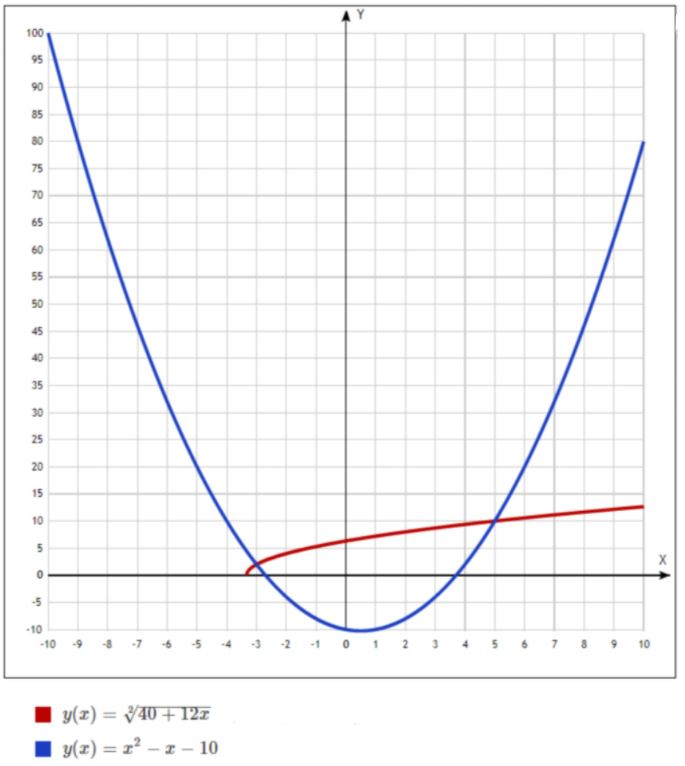
\includegraphics[width=\linewidth]{79I-2}
        \end{figure}
    \end{minipage}
\end{minipage}}
{НаписанноеРешение}
{ВерныйОтвет}{Подсказка}
\end{problem}

\begin{problem}{Квадратные неравенства.}{9.1.2}{79I}{(лёгкая)}
{Решить квадратное неравенство $x^{2} - 10x + 16 \leqslant 0$.}
{НаписанноеРешение}
{ВерныйОтвет}{Подсказка}
\end{problem}

\begin{problem}{Квадратные неравенства.}{9.1.2}{79I}{(лёгкая)}
{Решить квадратное неравенство $-2x^{2} + 5x + 7 \geqslant 0$.}
{НаписанноеРешение}
{ВерныйОтвет}{Подсказка}
\end{problem}

\begin{problem}{Квадратные неравенства.}{9.1.2}{79I}{(лёгкая)}
{Решить квадратное неравенство $(1 - 5x)^{2} \geqslant (11 + 3x)^{2}$.}
{НаписанноеРешение}
{ВерныйОтвет}{Подсказка}
\end{problem}

\begin{problem}{Квадратные неравенства.}{9.1.2}{9I}{(лёгкая)}
{Найти наибольшее целое решение неравенства $x^{2} - (8 - x)(8 + x) \leqslant 65 + (x + 2)^{2}$.

}
{НаписанноеРешение}
{ВерныйОтвет}{Подсказка}
\end{problem}

\begin{problem}{Квадратные неравенства.}{9.1.2}{X}{(лёгкая)}
{Высота над землёй подброшенного вверх мяча меняется по закону $h(t) = 1{,}6 + 8t - 5t^{2}$, где $h$~--- высота в метрах, $t$~--- время в секундах, прошедшее с момента броска. Сколько секунд мяч будет находиться на высоте не менее 3 метров?}
{НаписанноеРешение}
{ВерныйОтвет}{Подсказка}
\end{problem}

\begin{problem}{Квадратные неравенства.}{9.1.2}{X red метод интервалов}{(лёгкая)}
{Решить неравенство: $\,(x^{2} + 3x + 1)(x^{2} + 3x - 3) \geqslant 5$.}
{НаписанноеРешение}
{ВерныйОтвет}{Подсказка}
\end{problem}

\begin{problem}{Квадратные неравенства.}{9.1.2}{X}{*}
{Решить неравенство: $\,\displaystyle\frac{-25}{(x + 6)^{2} - 7} \geqslant 0$.}
{НаписанноеРешение}
{ВерныйОтвет}{Подсказка}
\end{problem}

\begin{problem}{Квадратные неравенства.}{9.1.2}{X}{(лёгкая)}
{Из жизненного опыта известно, что если достаточно быстро вращать ведёрко с водой на верёвке в вертикальной плоскости, то вода не выльется. При вращении ведёрка сила давления воды на дно не постоянна: она максимальна в нижней точке и минимальна в верхней. Вода не выливается, если сила её давления на дно будет положительной во всех точках траектории, кроме, может быть, верхней, где она может быть равной нулю. Сила давления в верхней точке равна $\displaystyle P = m\left(\frac{v^{2}}{L} - g\right)$, где $m$~--- масса воды (в кг), $v$~--- скорость движения ведёрка (в м/с), $L$~--- длина верёвки в метрах, $g$~--- ускорение свободного падения (считаем, что $g = 10$м/с$^{2}$).\\ С какой наименьшей скоростью надо вращать ведёрко, чтобы вода не выливалась, если длина верёвки равна 90 см?}
{НаписанноеРешение}
{ВерныйОтвет}{Подсказка}
\end{problem}

\begin{problem}{Доказательство неравенств. Неравенство КБШ.}{9.1.3}{9D OMMO}{(лёгкая)}
{Что больше: $1$ или $\frac{18}{71} + \frac{47}{187} + \frac{59}{117}$?}
{НаписанноеРешение}
{ВерныйОтвет}{Подсказка}
\end{problem}

\begin{problem}{Доказательство неравенств. Неравенство КБШ.}{9.1.3}{9D}{(лёгкая)}
{Что больше: $e^e \cdot \pi^{\pi}$ или $e^{2\pi}$?}
{НаписанноеРешение}
{ВерныйОтвет}{Подсказка}
\end{problem}

\begin{problem}{Доказательство неравенств. Неравенство КБШ.}{9.1.3}{9D}{(лёгкая)}
{Доказать, что неравенство $t + \frac1t \geqslant 2$ выполнено для любых $t > 0$.\\ Найти, при каком (каких) $t$ достигается равенство.}
{НаписанноеРешение}
{ВерныйОтвет}{Подсказка}
\end{problem}

\begin{problem}{Доказательство неравенств. Неравенство КБШ.}{9.1.3}{9D}{(лёгкая)}
{Доказать, что $x^{4} - 4x^{3} + 12x^{2} - 16x + 24 > 0$ для всех значений $x$.}
{НаписанноеРешение}
{ВерныйОтвет}{Подсказка}
\end{problem}

\begin{problem}{Доказательство неравенств. Неравенство КБШ.}{9.1.3}{9D}{(лёгкая)}
{Доказать, что $\displaystyle x^{2} + 49 \geqslant 14x$.}
{$x^2 + 49 \geqslant 14x \;\Leftrightarrow\; x^2 - 14x + 49 \geqslant 0 \;\Leftrightarrow\; (x - 7)^2 \geqslant 0$. Поскольку последнее неравенство очевидно является верным, верны и все неравенства, получаемые из него. Исходное неравенство доказано.}
{Смотри рассуждения выше. $(x - 7)^2 \geqslant 0$.}{Преобразуй данное неравенство к одному из опорных неравенств.}
\end{problem}

\begin{problem}{Доказательство неравенств. Неравенство КБШ.}{9.1.3}{9D}{(лёгкая)}
{Доказать, что $\displaystyle 2m^{2} - 12m + 20 \geqslant 0$ (для всех значений $m$)}
{$2m^{2} - 12m + 20 \geqslant 0 \;\Leftrightarrow\; m^2 - 6m + 10 \geqslant 0 \;\Leftrightarrow\; (m - 3)^2 + 1 \geqslant 0$. Поскольку последнее неравенство всегда верно (более того, верным является и строгое неравенство), верны и все неравенства, получаемые из него. Доказано.}
{Смотри рассуждения выше. $(m - 3)^2 + 1 > 0$.}{Для приведения к опорному неравенству выдели полный квадрат.}
\end{problem}

\begin{problem}{Доказательство неравенств. Неравенство КБШ.}{9.1.3}{X}{(лёгкая)}
{Доказать, что неравенство $37a^{2} - 12a - 2ab + b^{2} + 2 > 0$ выполняется при всех действительных значениях $a$ и $b$.}
{Для доказательства данного неравенства выделим полные квадраты. $$37a^{2} - 12a - 2ab + b^{2} + 2 = a^2 - 2ab + b^2 + 36a^2 - 12a + 1 + 1 = (a - b)^2 + (6a - 1)^2 + 1.$$ Поэтому $37a^{2} - 12a - 2ab + b^{2} + 2 > 0 \;\Leftrightarrow\; (a - b)^2 + (6a - 1)^2 + 1 > 0$.\\ Но так как квадрат любого вещественного числа неотрицателен, выражение в левой части неравенства не меньше 1, и данное неравенство верно для любых вещественных чисел $a$ и $b$.}
{Смотри рассуждения выше: левая часть неравенства не меньше 1.}{Выдели полные квадраты.}
\end{problem}

\begin{problem}{Доказательство неравенств. Неравенство КБШ.}{9.1.3}{9D}{(лёгкая)}
{Доказать, что $a^2 + b^2 + 1 > ab + a + b$.}
{НаписанноеРешение}
{ВерныйОтвет}{Подсказка}
\end{problem}

\begin{problem}{Доказательство неравенств. Неравенство КБШ.}{9.1.3}{X}{(не лёгкая)}
{Известно, что существует несколько разных средних, а именно следующие:
\begin{multline*}
\begin{aligned}
&\text{1) среднее арифметическое, } m = \frac{a + b}{2} \qquad \left(m = \frac{x_1 + x_2 + \ldots + x_n}{n}\right) \\
&\text{2) среднее геометрическое, } \;\;g = \sqrt{ab} \;\:\qquad\qquad \left(g = \sqrt[n]{x_1x_2\ldots x_n}\right) \\
&\text{3) среднее квадратическое, } s = \sqrt{\tfrac{a^2 + b^2}{2}} \:\quad\qquad \left(s = \sqrt{\tfrac{x_1^2 + x_2^2 + \ldots + x_n^2}{n}}\right) \\
&\text{4) среднее гармоническое, } \;\; h = \frac{2}{\frac1a + \frac1b} \qquad\qquad \left(h = \tfrac{n}{\frac{1}{x_1} + \frac{1}{x_2} +\ldots + \frac{1}{x_n}}\right)
\end{aligned}
\end{multline*}
Показать, что для любых положительных чисел верно {\large $\;s \geqslant m \geqslant g \geqslant h$}.\smallskip\\
То есть, доказать все три неравенства $\;\:\sqrt{\tfrac{a^2 + b^2}{2}} \:\geqslant\: \frac{a + b}{2} \:\geqslant\: \sqrt{ab} \:\geqslant\: \frac{2}{\frac1a + \frac1b}$.}
{Достаточно доказать неравенства $s \geqslant m$, $m \geqslant g$ и $g \geqslant h$.\smallskip\\
1) Неравенство между средним арифметическим и средним геометрическим.\\
$\frac{a + b}{2} \geqslant \sqrt{ab} \;\Leftrightarrow\; a + b \geqslant 2\sqrt{ab}$. Так как все числа положительны, можно смело возводить обе части в квадрат --- знак неравенства не изменится: $a + b \geqslant 2\sqrt{ab} \;\Leftrightarrow\; a^2 + 2ab + b^2 \geqslant 4ab \;\Leftrightarrow\; a^2 - 2ab + b^2 \geqslant 0 \;\Leftrightarrow\; (a - b)^2 \geqslant 0$. Очевидно, что последнее неравенство всегда верно, причем \textbf{равенство достигается только при $a = b$.} Доказано.\smallskip\\
2) Неравенство между средним квадратическим и средним арифметическим.\\
$\sqrt{\tfrac{a^2 + b^2}{2}} \geqslant \frac{a + b}{2} \;\Leftrightarrow\; \tfrac{a^2 + b^2}{2} \geqslant \frac{(a + b)^2}{4}$ (знак неравенства при возведении в квадрат не меняется --- числа положительны) $\tfrac{a^2 + b^2}{2} \geqslant \frac{(a + b)^2}{4} \;\Leftrightarrow\; 2a^2 + 2b^2 \geqslant a^2 + 2ab + b^2 \;\Leftrightarrow\; a^2 - 2ab + b^2 \geqslant 0 \;\Leftrightarrow\; (a - b)^2 \geqslant 0$. Очевидно, что последнее неравенство всегда верно, причем \textbf{равенство достигается только при $a = b$.} Доказано.\smallskip\\
3) Неравенство между средним геометрическим и средним гармоническим.\\
Для начала отметим, что $\frac{2}{\frac1a + \frac1b} = \frac{2}{\frac{b + a}{ab}} = \frac{2ab}{a + b}$. Тогда
$\;\sqrt{ab} \geqslant \frac{2}{\frac1a + \frac1b} \;\Leftrightarrow\; \sqrt{ab} \geqslant \frac{2ab}{a + b} \;\Leftrightarrow\;$ $ab \geqslant \frac{4a^2b^2}{(a + b)^2}$ (знак неравенства при возведении в квадрат не меняется). Далее, можно поделить обе части неравенства на $ab$ (положительное число, знак неравенства не поменяется) и домножить на $(a + b)^2$ (также положительное). Тогда получается эквивалентное неравенство $a^2 + 2ab + b^2 \geqslant 4ab \;\Leftrightarrow\; a^2 - 2ab + b^2 \geqslant 0 \;\Leftrightarrow\; (a - b)^2 \geqslant 0$. Очевидно, что последнее неравенство всегда верно, причем \textbf{равенство достигается только при $a = b$.} Доказано.}
{Доказательство всех трёх неравенств смотри выше. Равенство во всех этих неравенствах достигается одновременно --- тогда, когда числа равны.}{Если обе части неравенства положительны, то при возведении в квадрат знак неравенства сохраняется, а неравенство остаётся эквивалентным предыдущему.}
\end{problem}

\begin{problem}{Доказательство неравенств. Неравенство КБШ.}{9.1.3}{9D}{(лёгкая)}
{Определить отношение двух чисел, если отношение их среднего арифметического к среднему геометрическому равно $25{:}24$.}
{НаписанноеРешение}
{ВерныйОтвет}{Подсказка}
\end{problem}

\begin{problem}{Доказательство неравенств. Неравенство КБШ.}{9.1.3}{9D}{(лёгкая)}
{Доказать, что при любом $a$ имеет место неравенство $3(1 + a^2 + a^4) \geqslant (1 + a + a^2)^2$.}
{НаписанноеРешение}
{ВерныйОтвет}{Подсказка}
\end{problem}

\begin{problem}{Доказательство неравенств. Неравенство КБШ.}{9.1.3}{9D https://www.problems.ru/view_problem_details_new.php?id=35532}{(лёгкая)}
{Автобус называется переполненным, если в нём более 50 пассажиров. По дороге едет колонна автобусов (среди которых есть переполненные). Что больше --- процент переполненных автобусов или процент пассажиров, которые едут в переполненных автобусах?}
{Окрасим переполненные автобусы в красный цвет. В каждом автобусе изменим (уменьшим или увеличим) число так, чтобы их стало ровно 50. Теперь во всех автобусах поровну пассажиров, то есть процент красных автобусов стал равен проценту пассажиров в красных автобусах. Но так как из красных автобусов мы пассажиров удаляли, а в остальные --- добавляли, то изначально в красных автобусах процент пассажиров был больше чем процент красных автобусов.}
{ВерныйОтвет}{Подсказка}
\end{problem}

\begin{problem}{Доказательство неравенств. Неравенство КБШ.}{9.1.3}{9D}{(лёгкая)}
{Пусть $a$ и $b$ --- положительные числа. Показать, что верно неравенство: $$\frac{a + b}{a^2 + b^2} \leqslant \frac{1}{2a} + \frac{1}{2b}.$$}
{НаписанноеРешение}
{ВерныйОтвет}{Подсказка}
\end{problem}

\begin{problem}{Доказательство неравенств. Неравенство КБШ.}{9.1.3}{9D}{(лёгкая)}
{Доказать для положительных чисел неравенство $\frac{a_1}{a_2} + \frac{a_2}{a_3} + \ldots + \frac{a_n}{a_1} \geqslant n$.\smallskip\\
Используй неравенство между $m = \frac{x_1 + x_2 + \ldots + x_n}{n}$ и $g = \sqrt[n]{x_1x_2\ldots x_n}$.}
{НаписанноеРешение}
{ВерныйОтвет}{Подсказка}
\end{problem}

\begin{problem}{Доказательство неравенств. Неравенство КБШ.}{9.1.3}{9D}{(лёгкая)}
{Доказать, что для произвольного треугольника с известными сторонами $a$, $b$, $c$, и периметром $P$ выполнено следующее неравенство: $\;\frac{P}{a} + \frac{P}{b} + \frac{P}{c} \geqslant 9$.}
{НаписанноеРешение}
{ВерныйОтвет}{Подсказка}
\end{problem}

\begin{problem}{Доказательство неравенств. Неравенство КБШ.}{9.1.3}{9D https://www.problems.ru/view_problem_details_new.php?id=116991}{(лёгкая)}
{Найти наибольшее значение выражения $ab + bc + ac + abc$, если $a + b + c = 12$  (при этом известно, что $a$, $b$ и $c$ --- неотрицательные числа).}
{НаписанноеРешение}
{ВерныйОтвет}{Подсказка}
\end{problem}

\begin{problem}{Доказательство неравенств. Неравенство КБШ.}{9.1.3}{9D https://www.problems.ru/view_problem_details_new.php?id=73717}{(лёгкая)}
{Доказать, что если $a$, $b$, $c$ --- положительные числа, то верно неравенство: $$\;\frac{a}{b + c} + \frac{b}{a + c} + \frac{c}{a + b} \geqslant \frac32.$$}
{НаписанноеРешение}
{ВерныйОтвет}{Подсказка}
\end{problem}

\begin{problem}{Доказательство неравенств. Неравенство КБШ.}{9.1.3}{9D}{*}
{Пусть $a$, $b$, $c$ --- положительные числа. Показать, что верно неравенство: $$\frac{a + b}{a^2 + b^2} + \frac{b + c}{b^2 + c^2} + \frac{a + c}{a^2 + c^2} \leqslant \frac1a + \frac1b + \frac1c.$$}
{НаписанноеРешение}
{ВерныйОтвет}{Подсказка}
\end{problem}

\begin{problem}{Доказательство неравенств. Неравенство КБШ.}{9.1.3}{9D}{(лёгкая)}
{Доказать, что $\:\displaystyle 2013^{2015} \cdot 2015^{2013} < 2014^{2\cdot2014}$.}
{НаписанноеРешение}
{ВерныйОтвет}{Подсказка}
\end{problem}

\begin{problem}{Доказательство неравенств. Неравенство КБШ.}{9.1.3}{9D}{(лёгкая)}
{Доказать, что $\:\displaystyle \lg (n + 1) > \frac{\lg1 + \lg 2 + \ldots + \lg n}{n}$.}
{НаписанноеРешение}
{ВерныйОтвет}{Подсказка}
\end{problem}

\begin{problem}{Доказательство неравенств. Неравенство КБШ.}{9.1.3}{9D}{(лёгкая)}
{Доказать, что если $a + b = 1$, то имеет место неравенство $\:\displaystyle a^8 + b^8 > \tfrac{1}{128}$.}
{НаписанноеРешение}
{ВерныйОтвет}{Подсказка}
\end{problem}

\begin{problem}{Доказательство неравенств. Неравенство КБШ.}{9.1.3}{9D}{(лёгкая)}
{Доказать, что при $|x| < 1$ и $|y| < 1$ верно следующее неравенство: $\:\displaystyle\left|\frac{x - y}{1 - xy}\right| < 1$.}
{НаписанноеРешение}
{ВерныйОтвет}{Подсказка}
\end{problem}

\begin{problem}{Доказательство неравенств. Неравенство КБШ.}{9.1.3}{9D}{(лёгкая)}
{Даны положительные числа $a_1$, $a_2$, ..., $a_n$. Известно, что $a_1 + a_2 + \ldots + a_n \leqslant \frac12$. Докажите, что $(1 + a_1)\cdot(1 + a_2)\cdot\ldots\cdot(1 + a_n) < 2$.}
{НаписанноеРешение}
{ВерныйОтвет}{Подсказка}
\end{problem}

\begin{problem}{Доказательство неравенств. Неравенство КБШ.}{9.1.3}{9D}{(лёгкая)}
{Доказать, что если для чисел $a$, $b$ и $c$ выполняются неравенства $|a - b| \geqslant |c|$, $|b - c| \geqslant |a|$, $|c - a| \geqslant |b|$, то какое-то одно из этих чисел равно сумме двух других.

}
{НаписанноеРешение}
{ВерныйОтвет}{Подсказка}
\end{problem}

\begin{problem}{Доказательство неравенств. Неравенство КБШ.}{9.1.3}{9D red индукция, оценка сверху и снизу https://www.problems.ru/view_problem_details_new.php?id=66356}{*}
{Доказать, что среднее арифметическое всех делителей натурального числа $N$ лежит на отрезке $\left[\sqrt{N}, \:\frac{N + 1}{2}\right]$.}
{Для $n = 1$ отрезок вырождается в точку, утверждение будет верно. Далее считаем, что $n > 1$.
Пусть $k$ --- количество делителей числа  $n = a^2$.\smallskip\\
Оценка сверху. Количество собственных делителей равно $k - 2$ и каждый из них не превосходит $n/2$. Значит, сумма всех делителей не больше чем
$\frac{n}{2} (k - 2) + n + 1 = \frac{nk}{2} + 1$. Следовательно, их среднее арифметическое не превосходит  $\frac{n}{2} + \frac{1}{k} \leqslant \frac{n}{2} + \frac{1}{2} = n + \frac{1}{2}$.\\
Оценка снизу. Пусть $d_1d_2 = n$ и $d_1 \neq d_2$, тогда, как известно, $d_1 + d_2 > 2\sqrt{d_1d_2} = 2a$. Все делители $n$ (кроме $a$, если число $a$ --- целое) разбиваются на такие пары. В любом случае $d_1 + d_2 + \ldots + d_k > ka$.  Значит, $\frac{1}{k} (d_1 + d_2 + \ldots + d_k) > a$.}
{ВерныйОтвет}{Подсказка}
\end{problem}

\begin{problem}{Доказательство неравенств. Неравенство КБШ.}{9.1.3}{9D red https://www.problems.ru/view_problem_details_new.php?id=65558}{*}
{Ваня задумал два положительных числа $x$ и $y$. Он записал числа $x + y$, $x - y$, $xy$ и $\frac{x}{y}$ и показал их Пете, но не сказал, какое число какой операцией получено.\\
а) Допустим, Петя увидел числа 2, 3, 9, 18. Какие числа мог задумать Ваня?\\
б) Доказать, что в подобной задаче Петя сможет однозначно восстановить $x$ и $y$, независимо от того, какие 4 числа он увидит.}
{Заметим, что $((x+y) + (x-y))/2 = (xy \cdot x/y)^{1/2}$. С помощью перебора найдём на доске пару чисел $a < b$, чьё среднее арифметическое равно среднему геометрическому оставшейся пары чисел $c$ и $d$. Ниже мы докажем, что такое разбиение единственно (с точностью до перестановки равных чисел), поэтому $a = x - y$, $b = x + y$, откуда $x = 1/2(a + b)$, $y = 1/2(b - a)$. Докажем единственность. Если в равенстве $(a+b)/2 = (cd)^{1/2}$ поменять местами два неравных числа из разных частей, то равенство нарушится: ведь одна из частей увеличится, а другая --- уменьшится. Поменять пары целиком тоже нельзя: отрицательное число не может стоять под корнем, а если все числа неотрицательны, то $(c+d)/2 \geqslant (cd)^{1/2} = (a+b)/2 \geqslant (ab)^{1/2}$, и равенство достигается, только когда все четыре числа равны, что невозможно: $x + y > x - y$.}
{ВерныйОтвет}{Подсказка}
\end{problem}

\end{document}